% LADAR RXC Parsing State Machine (Fixed Loops)
\documentclass[tikz, border=10pt]{standalone}
\usepackage{tikz}
\usepackage{amsmath}
\usetikzlibrary{automata, positioning, arrows.meta, calc, shapes.geometric}

\begin{document}
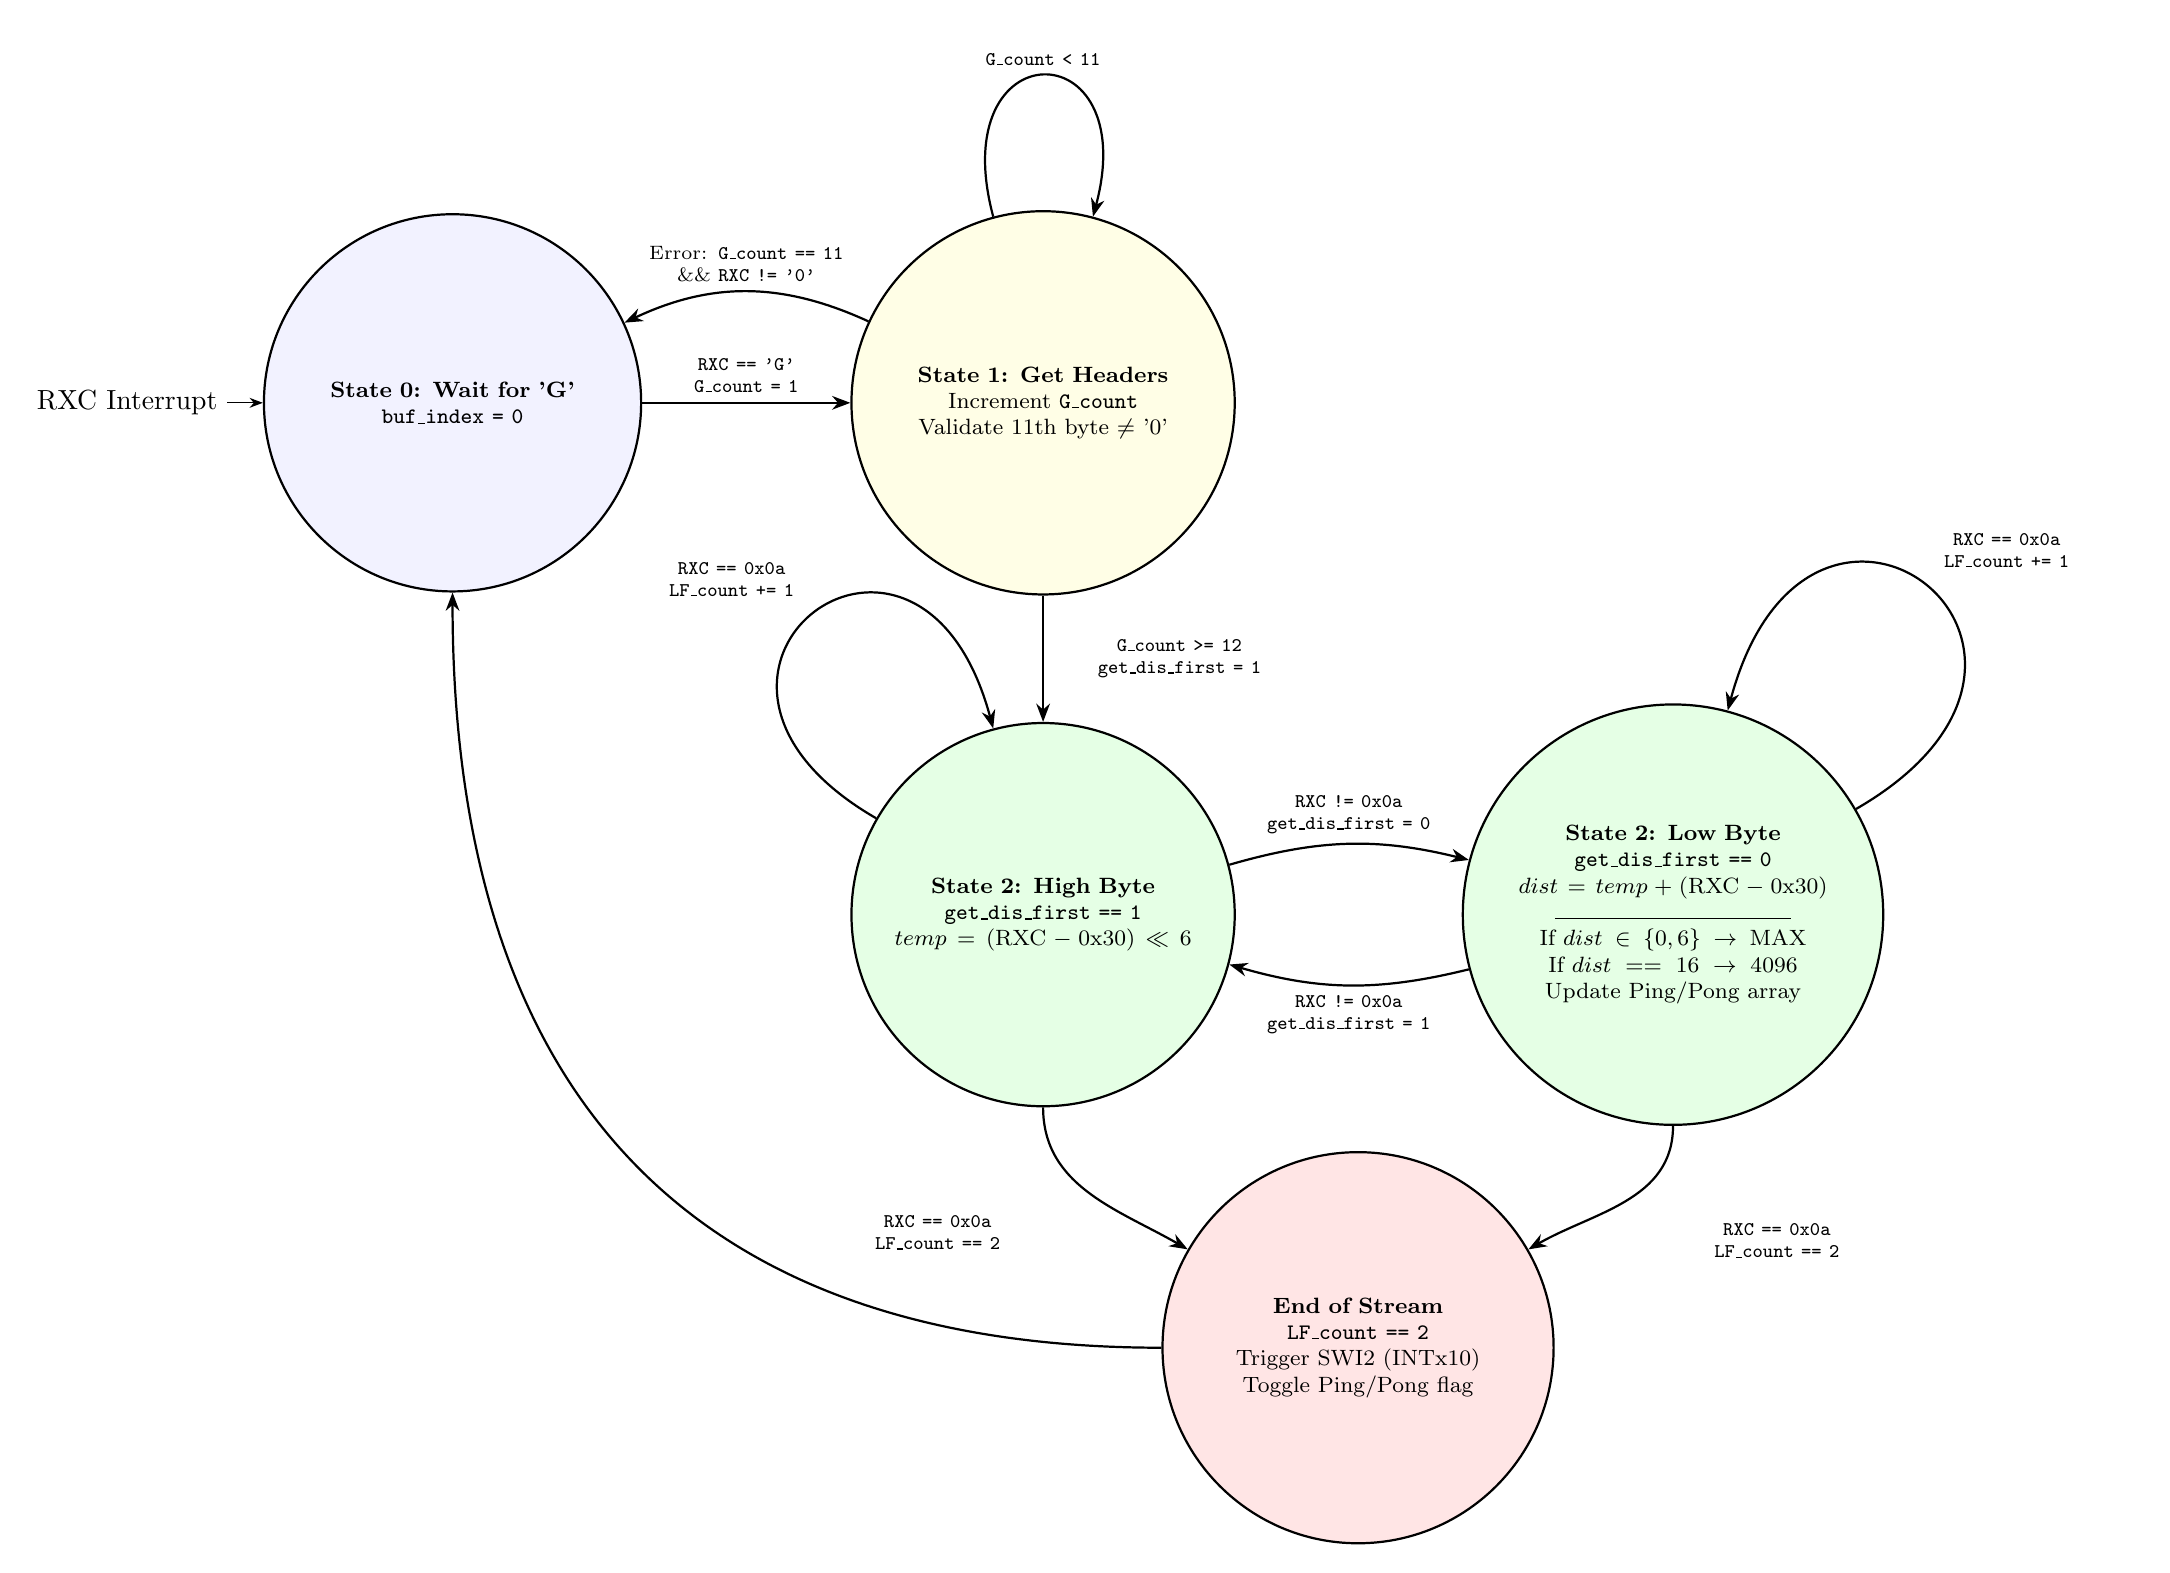
\begin{tikzpicture}[
    >=Stealth,
    node distance=5cm and 6cm, 
    on grid,
    auto,
    every state/.style={thick, fill=blue!5, text width=4.5cm, align=center, font=\footnotesize, minimum height=1.5cm},
    transition/.style={font=\scriptsize, align=center, text width=3.2cm}
]

% -------------------------
% STATES
% -------------------------
\node[state, initial, initial text={RXC Interrupt}] (WaitG) {
    \textbf{State 0: Wait for 'G'}\\ 
    \texttt{buf\_index = 0}
};

\node[state, fill=yellow!10] (Headers) [right=of WaitG, xshift=1.5cm] {
    \textbf{State 1: Get Headers}\\ 
    Increment \texttt{G\_count}\\
    Validate 11th byte $\neq$ '0'
};

\node[state, fill=green!10] (DataHi) [below=of Headers, yshift=-1.5cm] {
    \textbf{State 2: High Byte}\\ 
    \texttt{get\_dis\_first == 1}\\
    $temp = (\text{RXC} - 0\text{x}30) \ll 6$
};

\node[state, fill=green!10] (DataLo) [right=of DataHi, xshift=2cm] {
    \textbf{State 2: Low Byte}\\ 
    \texttt{get\_dis\_first == 0}\\
    $dist = temp + (\text{RXC} - 0\text{x}30)$\\
    \rule{3cm}{0.4pt}\\
    If $dist \in \{0,6\} \rightarrow \text{MAX}$\\
    If $dist == 16 \rightarrow 4096$\\
    Update Ping/Pong array
};

% Position EndStream midway between DataHi and DataLo, shifted down
\node[state, fill=red!10] (EndStream) at ($(DataHi)!0.5!(DataLo) + (0, -5.5cm)$) {
    \textbf{End of Stream}\\ 
    \texttt{LF\_count == 2}\\
    Trigger SWI2 (INTx10)\\
    Toggle Ping/Pong flag
};

% -------------------------
% TRANSITIONS
% -------------------------
% State 0 to 1
\path[->, thick]
(WaitG) edge node [transition, above] {\texttt{RXC == 'G'}\\ \texttt{G\_count = 1}} (Headers);

% State 1 loops and exits
\path[->, thick]
(Headers) edge [loop above, looseness=5] node [transition, above] {\texttt{G\_count < 11}} (Headers)
(Headers) edge [bend right=25] node [transition, above] {Error: \texttt{G\_count == 11}\\ \&\& \texttt{RXC != '0'}} (WaitG)
(Headers) edge node [transition, right] {\texttt{G\_count >= 12}\\ \texttt{get\_dis\_first = 1}} (DataHi);

% State 2 Data Ping-Pong (Hi/Lo bytes)
\path[->, thick]
(DataHi) edge [bend left=15] node [transition, above] {\texttt{RXC != 0x0a}\\ \texttt{get\_dis\_first = 0}} (DataLo)
(DataLo) edge [bend left=15] node [transition, below] {\texttt{RXC != 0x0a}\\ \texttt{get\_dis\_first = 1}} (DataHi);

% State 2 Line Feed Handling (Shifted to upper shoulders to avoid crossing lines)
\path[->, thick]
(DataHi) edge [out=150, in=105, loop, looseness=5] node [transition, above left=0.1cm and -0.7cm] {\texttt{RXC == 0x0a}\\ \texttt{LF\_count += 1}} (DataHi)
(DataLo) edge [out=30, in=75, loop, looseness=5] node [transition, above right=0.1cm and -0.7cm] {\texttt{RXC == 0x0a}\\ \texttt{LF\_count += 1}} (DataLo);

% End Stream Transitions
\path[->, thick]
(DataHi) edge [out=-90, in=150] node [transition, left, xshift=-0.2cm, yshift=-0.5cm] {\texttt{RXC == 0x0a}\\ \texttt{LF\_count == 2}} (EndStream)
(DataLo) edge [out=-90, in=30] node [transition, right, xshift=0.2cm, yshift=-0.5cm] {\texttt{RXC == 0x0a}\\ \texttt{LF\_count == 2}} (EndStream);

% Back to Start (Wraps cleanly, given a wider berth with in=-110 and looseness=1.2)
\path[->, thick]
(EndStream) edge [out=180, in=-90, looseness=1.2] node [transition, left, xshift=-0.2cm, yshift=-0.5cm] {} (WaitG);

\end{tikzpicture}
\end{document}